% Chapter 1

\chapter{Nonlinear FEM Framework in Orthogonal Basis} % Main chapter title

\label{Chapter3} % For referencing the chapter elsewhere, use \ref{Chapter1} 

%----------------------------------------------------------------------------------------
%----------------------------------------------------------------------------------------

\section{Continuum Mechanics and Kinematical Relations} \label{sec:continuum_kinematics}

\begin{figure}  
    \centering
    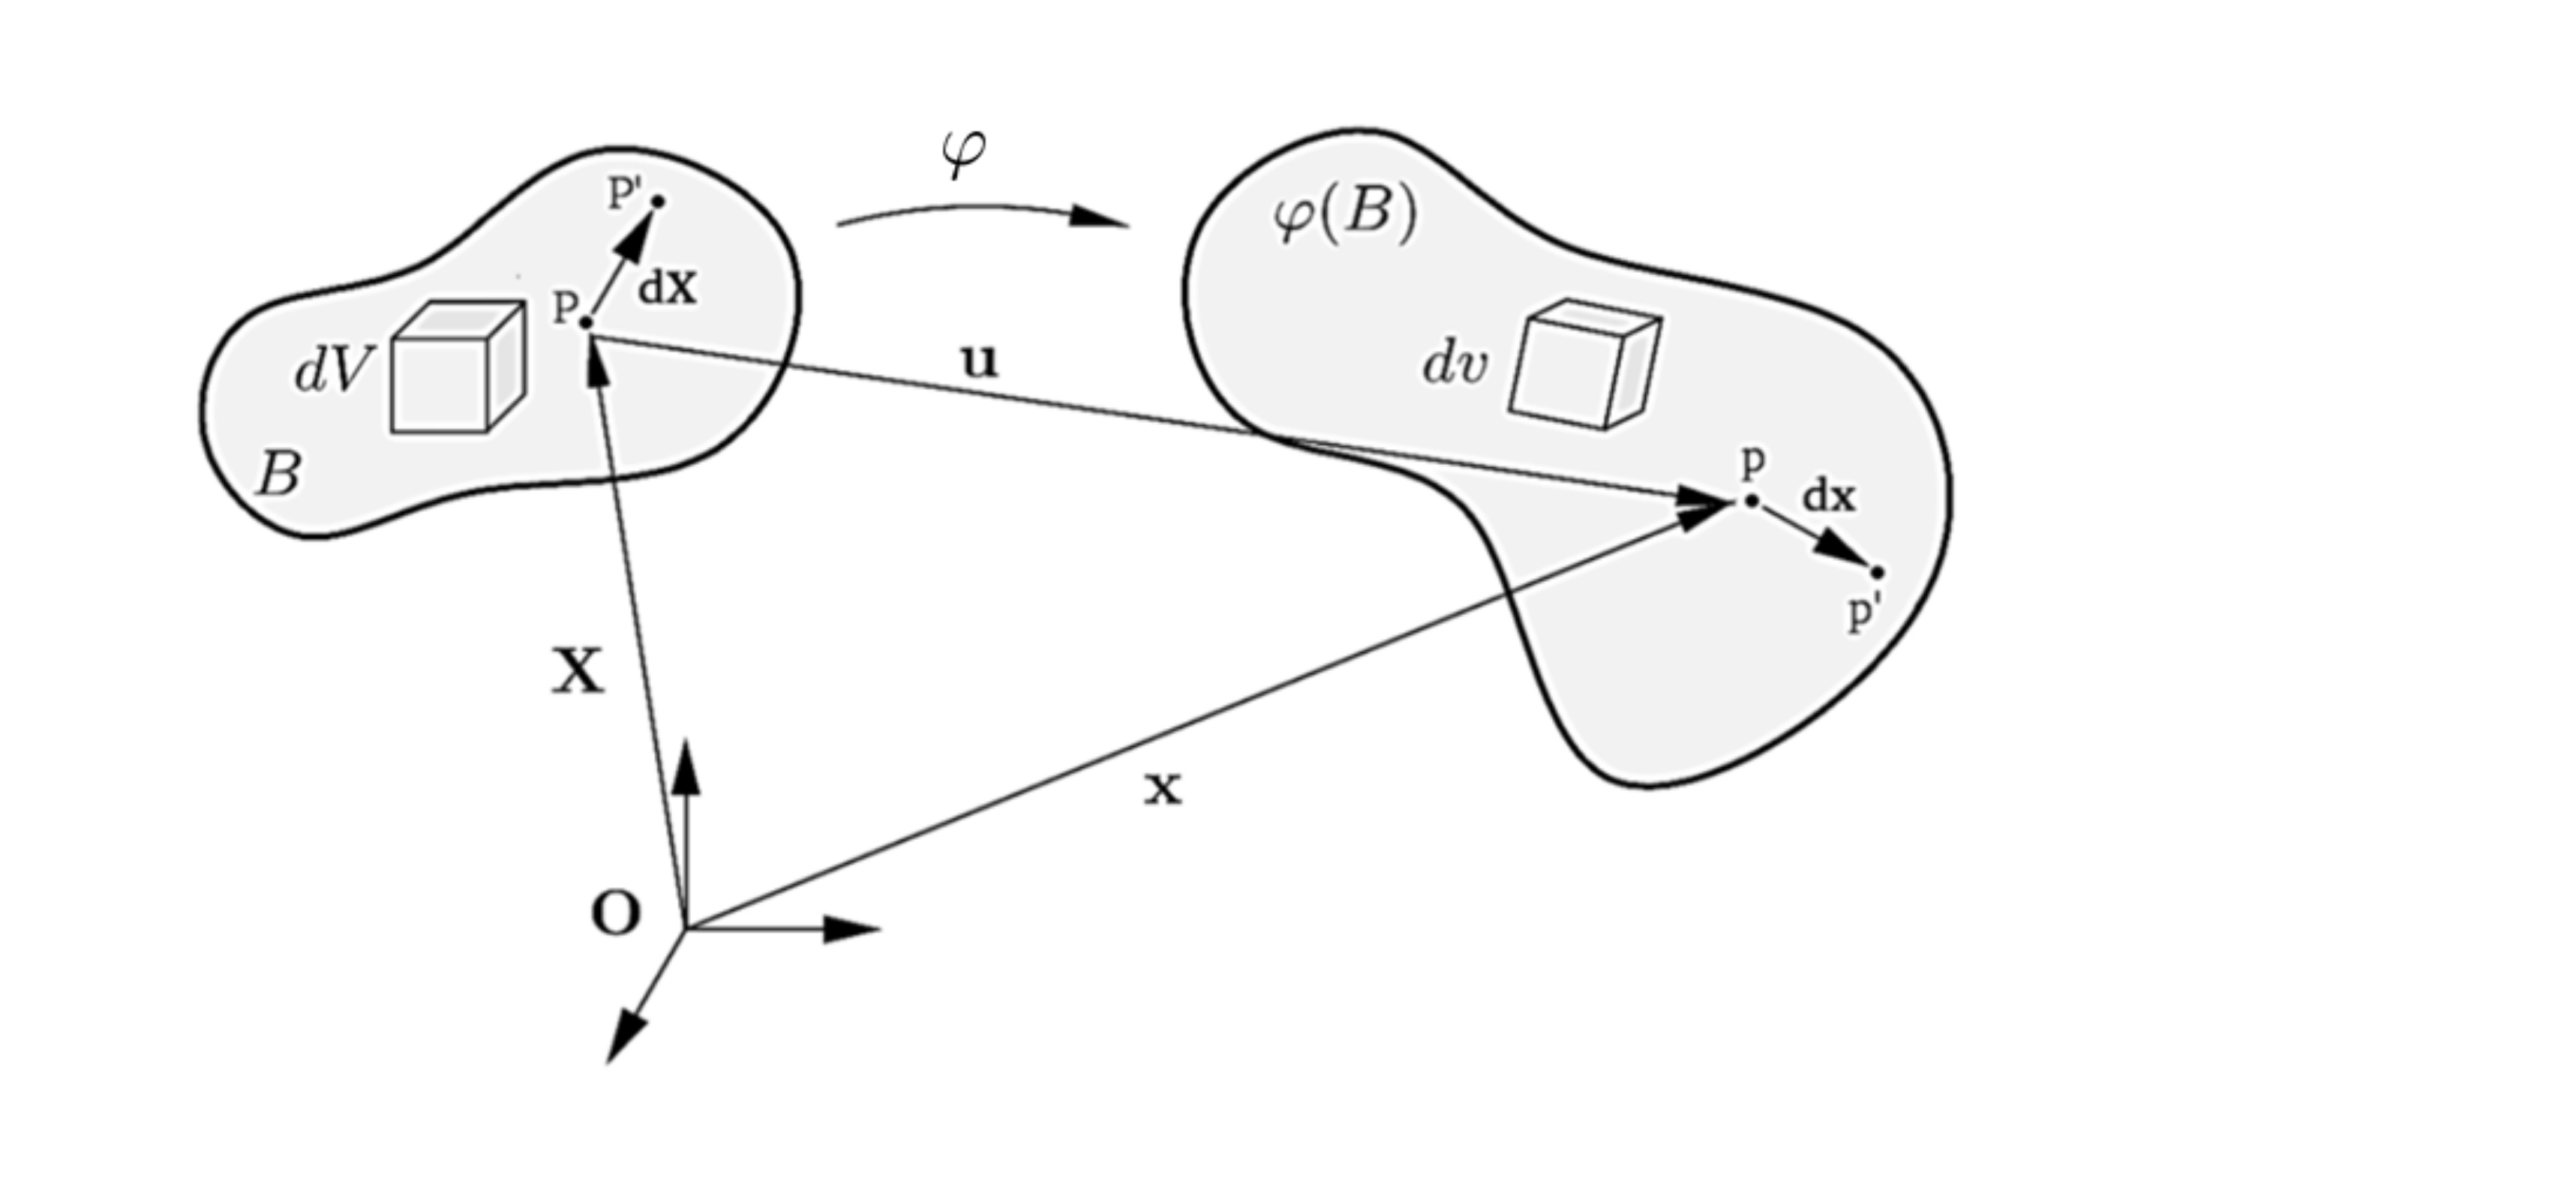
\includegraphics[scale = 0.60]{Images/ortho_map.png}
    \caption[Configuration and Motion of a Continuum Body in Orthogonal Basis]{Configuration and motion of a continuum body in orthogonal basis (Image Source: Institute of Applied Mechanics, RWTH Aachen).}
    \label{fig:km_config}
\end{figure}
According to continuum mechancis, a body $\mathcal{B}$ is defined as a manifold consisting of finite number of particles.
 This body $\mathcal{B}$ is also assumed to be a $\sigma-\text{finite measure space}$ - 
 this implies that each subset of $\mathcal{B}$ is associated with a non-negative measure, 
 which in this case would be the mass distribution.
 This manifold is assumed to be smooth, sufficiently differentiable, and the configuration of the particales at a given time
 can be mapped one-to-one onto Euclidean space, $\varphi: \mathcal{B} \rightarrow \mathbb{E}^{3}$, thus assigning a position vector to 
 each particle of the body in $\mathbb{E}^{3}$ \cite{truesdell2012,wriggers2008}. For simplicity, an orthogonal cartesian basis is assumed in this section as
 the formulation will be based on isoparametric interpolations - which rely on an orthogonal basis. A more general
 description using curvilinear coordinates is covered in Section \ref{sec:curvy_coords}. 
In order to ease the description of motion and deformation, it is convenient to assume a \emph{reference configuration}
 at an fixed time $t = t_{0}$. In this configuration, the body is assumed to be unloaded, undeformed, and unstressed.
 For an arbitrary point on the body $\mathrm{P}$ a position vector can be defined with respect to the origin of the basis,
\begin{equation}\label{ref_config_defition}
    \begin{cases}
        \boldsymbol{X} &= \boldsymbol{\varphi}(X, t_{0}),\\
        \boldsymbol{X} &= X^{i} \, \boldsymbol{E}_{i}\, , \, \, \text{where } {X}^{i}: {X}^{1}, {X}^{2}, {X}^{3} 
    \end{cases}
    \end{equation}
and $\boldsymbol{E}_{i}$ are unit vectors along the ${X}^{i}$ axes.

At any other time \emph{t} the configuration of the body will be referred to as the \emph{current configuration}.
 This mapping of the reference configuration into the current configuration is assumed to be so that all points in
 both configurations are mapped one-to-one. The position vector of the point $\mathrm{P}$
 that has now moved due to external forces to a position $\mathrm{p}$ can be defined as
\begin{equation} \label{curr_config_definition}
    \begin{cases}
        \boldsymbol{{x}} &= \boldsymbol{\varphi_{t}}(\boldsymbol{X}, t), \\
        \boldsymbol{{x}} &= {x}^{i} \, \boldsymbol{{e}}_{{i}}\, , \, \, \text{where } {x}^{i}: {x}^{1}, {x}^{2}, {x}^{3}.
    \end{cases}
\end{equation}
Similarly, $\boldsymbol{{e}}_{{i}}$ are the unit vectors
 along the ${x}^{i}$ axes.

Two consequences follow the assumption of a cartesian basis system. The dual basis to the unit vectors $\boldsymbol{{E}}_{{i}}$ and $\boldsymbol{{e}}_{{i}}$
 reduces to the original basis, thus making the position of the indices immaterial. Furthermore, as $\boldsymbol{E}$ and $\boldsymbol{e}$ are self adjoint,
 it can be shown that $\boldsymbol{{E}}_{{i}} = \boldsymbol{{E}}^{{i}} = \boldsymbol{{e}}_{{i}} = \boldsymbol{{e}}^{{i}}$, thus making the unit
 vectors and the position of the indices in both the configurations interchangeable without any effects to the maths involved.
The position vector of the point $\mathrm{p}$ relative to $\mathrm{P}$ is called the displacement vector $\boldsymbol{{u}}$ and can be defined as
\begin{equation} \label{displacement_vector}
    \boldsymbol{{u}} = \boldsymbol{{x}} - \boldsymbol{{X}} = {U}^{{i}} \boldsymbol{{E}}_{{i}} = {u}^{{i}} \boldsymbol{{e}}_{{i}}.
\end{equation}
In the reference configuration an infinitesimal vectorial line element between two points can be written as $\mathrm{d}\boldsymbol{X}$.
 Similarly, $\mathrm{d}\boldsymbol{x}$ can be defined as the infinitesimal vectorial line element between the corresponding points in the current configuration.
 The mapping from $\mathrm{d\boldsymbol{X}}$ to $\mathrm{d\boldsymbol{x}}$ can be used to study the deformation of the body. This
 mapping can be represented with the help of a second order tensor called the \emph{deformation gradient}.
 \begin{gather} \label{deformation_gradient}
    \mathrm{d}\boldsymbol{x} = \boldsymbol{{F}} \, \mathrm{d}\boldsymbol{X} \\
    \boldsymbol{{F}} := \mathrm{Grad} \, \boldsymbol{{x}} = \frac{\partial \boldsymbol{{x}}}{\partial \boldsymbol{{X}}^{{i}}} \otimes \boldsymbol{{e}}^{{i}} = \frac{\partial{x}^{i}}{\partial {X}^{{j}}} \, \boldsymbol{{e}}_{{i}} \otimes \boldsymbol{{e}}^{{j}} = {F}^{{i}}_{.j} \, \boldsymbol{e}_{i} \otimes \boldsymbol{e}^{j} 
\end{gather}
The deformation gradient further allows the transformation of differential quantities from the reference to the current configuration.
 A differential area element $\mathrm{d}\boldsymbol{a}$ in the current configuration can be written in terms of the area element $\mathrm{d}\boldsymbol{A}$ in the reference configuration
 using Nanson's formula,
 \begin{equation} \label{Nansons}
    \mathrm{d}\boldsymbol{a} = \mathbf{n} \,da = J \boldsymbol{F}^{-T} \boldsymbol{N} \,dA = J \boldsymbol{F}^{-T} \mathrm{d}\boldsymbol{A},
 \end{equation}
 where $\boldsymbol{n}$ and $\boldsymbol{N}$ are the normal vectors of the area elements $\mathrm{d}\boldsymbol{a}$ and $\mathrm{d}\boldsymbol{A}$ respectively, and $J$ is the determinant of the deformation gradient
 \begin{equation}\label{jacobian_deformation_gradient}
    J = \det\boldsymbol{F}.
 \end{equation}
 This also enables us to construct a relation between the differential volume elements,
 \begin{equation} \label{volume}
    dv = J\,dV.
 \end{equation}
The squares of the line elements $\mathbf{d}\boldsymbol{x}$ and $\mathbf{d}\boldsymbol{X}$ are related with the use of the right and left \emph{Cauchy-Green tensors} represented as $\boldsymbol{C}$ and
 $\boldsymbol{b}$ respectively, that are defined as,
\begin{align} \label{cauchy_green_tensors}
    \mathrm{d}\boldsymbol{x} \cdot \mathrm{d}\boldsymbol{x} &= \mathrm{d}\boldsymbol{X} \cdot \boldsymbol{C} \mathrm{d}\boldsymbol{X}, \text{ where } \boldsymbol{C} := \boldsymbol{F}^{T}\boldsymbol{F},\\
    \mathrm{d}\boldsymbol{X} \cdot \mathrm{d}\boldsymbol{X} &= \mathrm{d}\boldsymbol{x} \cdot \boldsymbol{b}^{-1} \mathrm{d}\boldsymbol{x}, \text{ where } \boldsymbol{b} := \boldsymbol{F} \boldsymbol{F}^{T},
\end{align}
which enables us to define the strain measures based on the difference between the squared lengths
 $\Vert\mathrm{d}\boldsymbol{x} \cdot \mathrm{d}\boldsymbol{x}\Vert^{2} - \Vert\mathrm{d}\boldsymbol{X} \cdot \mathrm{d}\boldsymbol{X}\Vert^{2} $, known as the \emph{Green-Lagrange strain tensor} and the \emph{Almansi strain tensor} respectively
\begin{align} \label{strain_measures}
    \boldsymbol{E} &:= \frac{1}{2} \left(\boldsymbol{C} - \boldsymbol{I}\right),\\
    \boldsymbol{e} &:= \frac{1}{2} \left(\boldsymbol{I} - \boldsymbol{b}^{-1}\right).
\end{align}
\section{Stress and Balance Equations}
On a body $\mathcal{B}$, the Cauchy stress vector $\mathbf{t}$ refers to a force per unit area of the deformed surface with a unit normal vector
\begin{equation} \label{traction_vector_definition}
    \mathbf{t} = \lim_{\Delta a \rightarrow 0} \frac{\mathbf{\Delta p}}{\Delta a}. 
\end{equation}
According to the \emph{Cauchy postulate}, the stress vector $\mathbf{t}$ is only dependent on the unit normal $\mathbf{n}$ and not on any other characteristic
 of the surface. This mapping between the stress vector and the unit normal can be represented with the help of a second order tensor called the \emph{Cauchy stress tensor}
 \begin{equation} \label{cauchy_stress_tensor}
    \mathbf{t} = \boldsymbol{\sigma} \mathbf{n}, \text{ where } \boldsymbol{\sigma} = \sigma^{ij} \mathbf{e}_{i} \otimes \mathbf{e}_{j}.
 \end{equation}

The fundamental relations of continuum mechanics are the balance relations.
 They are stated in the following briefly and without proof. The derivations can be found in \cite{wriggers2008} and \cite{itskov2020}.
\subsection{Balance of Mass}
For a closed system, the total mass is conserved i.e. over a given period of time, the change in mass ($\dot{m}$) is zero.
 This implies that the mass of the body in the reference configuration is equal to the 
 mass of the body in the current configuration.
\begin{align}\label{mass_balance}
    \dot{m} &= 0,\\
    \rho \, dv &= \rho_{0} \, dV,
\end{align}
where $\rho$ and $dv$ are the mass density and the volume of the body in the current configuration, and 
 $\rho_{0}$ and $dV$ are the density and volume of the body in the reference configuration.
\subsection{Balance of Linear Momentum}
The rate of change of linear momentum of a body is equal to the sum of the external forces acting on the body.
\begin{equation}\label{lin_momentum_balance}
    \begin{cases}
        \mathrm{div} \boldsymbol{\sigma} + \boldsymbol{f} = \rho \, \boldsymbol{\ddot{x}},\\
        \sigma ^{ij}||_{j} + f^{i} = \rho \, a^{i},
    \end{cases}  
\end{equation}
where $\boldsymbol{f}$ is the sum of forces acting on a body excluding inertia, $\boldsymbol{a} := \boldsymbol{\ddot{x}} = a^{i} \boldsymbol{e}_{i}$
 is the acceleration of a particle with the position vector $\boldsymbol{x}$.
The First Piola-Kirchhoff stress tensor can be used to represent the linear momentum balance in the reference configuration that can be written as
\begin{equation}\label{lin_momentum_balance_refconfig}
    \begin{cases}
        \mathrm{Div} \boldsymbol{{P}} + \boldsymbol{f}_{0} = \rho_{0} \, \boldsymbol{\ddot{x}},\\
        P^{ij}|_{j} + f_{0}^{i} = \rho_{0} \, a_{0}^{i}.\
    \end{cases}
\end{equation} 
In \eqref{lin_momentum_balance} and \eqref{lin_momentum_balance_refconfig}, the differential operators $(\bullet)|_{j}$
 and $(\bullet)||_{j}$ are the covariant derivatives in the current and the reference configurations respectively.
\subsection{Balance of Angular Momentum}
The rate of change of angular momentum of a body is equal to the resultant moment of the external forces acting on the body.
\begin{equation}\label{angular_momentum}
    \int_{\mathcal{B}} \rho(\boldsymbol{x}\, \times \boldsymbol{v}) = \int_{\mathcal{B}} \rho(\boldsymbol{x}\, \times \boldsymbol{b}) + \int_{\partial\mathcal{B}} (\boldsymbol{x}\, \times \boldsymbol{t}).
\end{equation}
This results in the local balance of angular momentum which simply requires the Cauchy stress tensor to be symmetric
\begin{align} \label{cauchy_stress_sym}
    \boldsymbol{\sigma} &= \boldsymbol{\sigma ^{T}},\\
    \sigma _{ij} &= \sigma _{ji}.
\end{align}
\subsection{Balance of Kinetic Energy}
An extension of \eqref{lin_momentum_balance}, is the balance of kinetic energy which states that the power of external forces $P$
 is equal to the sum of the stress power $W$ and the change in kinetic energy $\dot{K}$ of a body.
\begin{gather}\label{kin_energy}
    P = W + \dot{K},\\
    \int_{\mathcal{B}} \rho \,\boldsymbol{\overline{\mathrm{b}}} \cdot \boldsymbol{\mathrm{v}} \, dv + \int_{\partial \mathcal{B}} \boldsymbol{\mathrm{t}} \cdot \mathrm{\boldsymbol{v}} \, da =
    \int_{\mathcal{B}} \boldsymbol{\sigma} : \boldsymbol{\mathrm{d}} \,dv + \int_{\mathcal{B}} \frac{1}{2} \rho \mathrm{\boldsymbol{v}} \cdot \mathrm{\boldsymbol{v}} \, dv. \notag
\end{gather}
Represented by the Cauchy stress tensor, $\boldsymbol{\sigma}$, and the rate of deformation tensor, \textbf{d},
 the stress power can be decomposed further into heat production, $\mathcal{D}$ ad the stored energy density, $\Psi$, as follows
\begin{equation}\label{stress_power}
    W = \mathcal{D} + \int_{\mathcal{B}} \dot{\Psi}\,dV_{0}.
\end{equation} 
\subsection{Conservation of Energy}
The First Law of Thermodynamics states that the rate of change of the total energy $\dot{E}$ of a system is equal to the
 sum of the mechanical power of the external loads $P$ and the heat supplied $Q$ to the system.
\begin{gather}\label{first_thermo}
    \dot{E} = P + Q,\\
    \frac{\mathrm{d}}{\mathrm{dt}}\left[\int_{\mathcal{B}} \frac{1}{2} \rho \mathrm{\boldsymbol{v}} \cdot \mathrm{\boldsymbol{v}} \, dv + \int_{\mathcal{B}} \rho u \, dv\right] = 
    \int_{\mathcal{B}} \rho \,\boldsymbol{\overline{\mathrm{b}}} \cdot \boldsymbol{\mathrm{v}} \, dv + \int_{\partial \mathcal{B}} \boldsymbol{\mathrm{t}} \cdot \mathrm{\boldsymbol{v}} \, da - \int_{\partial \mathcal{B}} \boldsymbol{\mathrm{q}} \cdot \boldsymbol{\mathrm{n}} \, da + \int_{\mathcal{B}} \rho \, r \,dv, \notag
\end{gather}
where \textbf{q} and \textbf{n} are the heat flux vector and the surface normal respectively, and \emph{r} is the distributer inner heat source.
\section{Constitutive Relations}
Constitutive relations are the properties of the material under investigation. They characterise the material response of a body and
 are necessary to complete the system of differential equations for the solution of boundary value problems \cite{itskov2020}. Materials in the real world can exhibit incredibly diverse behaviours making it necessary for the constitutive relations to
 have a degree of approximation involved in their formulation. However, the relations must agree with the observed experimental behaviours. All constitutive relations must satisfy the 
 second law of thermodynamics and three general principles that are known as \emph{Noll's axioms}.
 These are the \emph{principle of determinism}, which states that the stress in a particular point can be determined by 
 the stress history at that point; the \emph{principle of local action},
 that states that the stress at a particular point is affected by the motion of the particles in
 immediate neighbourhood of that point; and the \emph{principle of material objectivity}, which states that the choice of coordinate
 system should not affect the material properties. 
Hyperelastic materials can be characterised by having zero heat dissipation. Thus the stress power \eqref{stress_power}
 reduces to
 \begin{equation}\label{hyper_stress_power}
    W = \int_{\mathcal{B}} \dot{\Psi}\,dV_{0}.
 \end{equation}
Comparing equations \eqref{kin_energy} and \eqref{hyper_stress_power}, according to \cite{itskov2020},
 \begin{gather}\label{S_is_Psi}
    \dot{\Psi} = \mathrm{J} \boldsymbol{\sigma} : \mathrm{\boldsymbol{d}} = \mathrm{\boldsymbol{S}} : \frac{1}{2}\mathrm{\boldsymbol{\dot{C}}} = 2 \frac{\partial \Psi}{\partial \mathrm{\boldsymbol{C}}} : \frac{1}{2} \mathrm{\boldsymbol{\dot{C}}}, \notag\\
    \therefore \, \mathrm{\boldsymbol{S}}  = 2 \frac{\partial \Psi}{\partial \mathrm{\boldsymbol{C}}}.
\end{gather}
Neo-Hookean materials are examples of hyperelastic materials. The model can be used to approximate the behaviour of
 rubber like materials fairly accurately for strains upto 20\% \cite{gent2001}. Given a Neo-Hookean material model defined as,
\begin{equation} \label{neo_hookean_definition}
{\boldsymbol{\sigma} = \frac{\mu}{J}\left(\boldsymbol{b}-\boldsymbol{I}\right) + \frac{\Lambda}{J}\ln{J}\boldsymbol{I}}
\end{equation}
The expression for the compliance matrix in the reference configuration can be written as

\begin{equation} \label{compliance_definition}
    {\mathbb{C} = 4\frac{\partial^2 \Psi}{\partial\boldsymbol{C}\partial\boldsymbol{C}} = 2\frac{\partial\boldsymbol{S}}{\partial\boldsymbol{C}}}
\end{equation}
 where \textbf{S} is the second Piola-Kirchhoff stress tensor which is defined as,
\begin{equation}\label{eq:19}
    {\boldsymbol{S} = J \boldsymbol{F^{-1} \sigma F^{-T}}}
\end{equation}
The given material model can be written using the Second Piola Kirchhoff Stress Tensor.
\begin{equation}\label{neo_hookean_S}
    {\boldsymbol{S} = \mu\left(\boldsymbol{I} - \boldsymbol{C^{-1}}\right) + \Lambda\ln{J}\boldsymbol{C^{-1}}}
\end{equation}
The compliance matrix is a fourth order tensor and using \eqref{neo_hookean_S} and \eqref{compliance_definition} can be written in the indicial form as follows
\begin{equation}\label{compliance_matrix_reference}
    \mathbb{C}^{i.a.}_{.j.b} = 2\left(-\mu + \Lambda\ln{J}\right)\left(C^{-1}\right)^i_{.a} \left(C^{-1}\right)^b_{.j} + \Lambda \left(C^{-1}\right)^i_{.j} \left(C^{-1}\right)^a_{.b}.
\end{equation}
Applying push-forward to \eqref{compliance_matrix_reference} to transform $\mathbb{C}$ to the current configuration,
\begin{equation} \label{compliance_matrix_current}
    \mathbbmss{c}^{i.a.}_{.j.b} = 2\left(-\mu + \Lambda\ln{J}\right) \delta^i_{.a} \delta^b_{.j} + \frac{\Lambda}{2} \delta^i_{.j} \delta^a_{.b}.
\end{equation}

\section{Weak Form}
Using the strong form of the linear momentum balance, \eqref{lin_momentum_balance},
 the weak form can be derived using a test function as described in Section \ref{sec:poisson_weak_form} and the contributions can be 
 separated into \emph{internal virtual work} and \emph{external virtual work}. A derivation of the weak form using
 general curvilinear coordinates can be found in Section \ref{sec:curvy_weak_form}, which can be reduced to obtain the following 
\begin{equation} \label{weak_form_beam}
    \underbrace{\int_{\mathcal{B}} \mathrm{grad}(\boldsymbol{w}) : \boldsymbol{\sigma} \,dv}_{\text{internal virtual work}} - 
        \underbrace{\int_{\mathcal{B}} \boldsymbol{w}\cdot \rho \overline{\boldsymbol{b}} \,dv - \int_{\partial_{t}\mathcal{B}} \boldsymbol{w} \cdot \overline{\boldsymbol{t}} \,da}_{\text{external virtual work}} = 0
\end{equation}
where the contributions of the internal virtual work and external virtual work can be defined as $G_{int}$ and $G_{ext}$ respectively.

\section{Discretisation} \label{sec:nonlinear_discretisation}
The reference configuration $\mathcal{S}_{0}$ is discretised into a set of finite elements, $\Omega_{0}^{e}$ that are defined by nodal points
 $\boldsymbol{X}$. Thus, the current configuration is composed by finite elements $\Omega^{e}$ with nodal points $\boldsymbol{x}$
 that are related to $\boldsymbol{X}_{I}$ through relations described in \ref{sec:continuum_kinematics}. 

After the discretisation of the domain into finite elements, the shape functions can be used to discretise the nodal variables
 in the reference and current configurations $\boldsymbol{X}$ and $\boldsymbol{x}$, the primary field variables $\boldsymbol{u}$,
 and the test functions $\boldsymbol{w}$ within each finite element can be discretised using the shape functions according to the isoparametric concept
 as described in Section \ref{sec:isoparametric_theory}. 
 Given a finite element domain, $\Omega$, and shape functions, $\boldsymbol{N}^{e}$,
 \begin{align} \label{nodal_discretisations}
    \boldsymbol{X} &\approx \boldsymbol{X}^{h} = \sum^{n_{en}}_{k=1} N^{e}_{k} X^{e}_{n} = \mathbf{N}^{e}\mathbf{X}^{e},\\
    \boldsymbol{x} &\approx \boldsymbol{x}^{h} = \sum^{n_{en}}_{k=1} N^{e}_{k} x^{e}_{n} = \mathbf{N}^{e}\mathbf{x}^{e},\\
    \boldsymbol{u} &\approx \boldsymbol{u}^{h} = \sum^{n_{en}}_{k=1} N^{e}_{k} u^{e}_{n} = \mathbf{N}^{e}\mathbf{u}^{e},\\
    \boldsymbol{w} &\approx \boldsymbol{w}^{h} = \sum^{n_{en}}_{k=1} N^{e}_{k} w^{e}_{n} = \mathbf{N}^{e}\mathbf{w}^{e},
 \end{align}
where the summation is carried over the $n_{en}$ nodes of the element. 
Using the above given definitions, and the weak form of the momentum balance \eqref{weak_form_beam}, the discretised form of the weak form
 in its internal virtual work contributions as summed over $n_{el}$ elements can be given as,
\begin{align} \label{discretised_g_int}
    G_{\text{int}} \approx G^{e}_{\text{int}} = \sum^{n_{el}}_{e=1} G^{e}_{\text{int}}, \,\,\text{where } \, \, G^{e}_{\text{int}} &= \int_{\Omega^{e}} \mathrm{grad}(\boldsymbol{w}) : \boldsymbol{\sigma} \,dv \notag\\
    \text{and }\,\, G^{e}_{int} &= \mathbf{w}^{T}_{e} \int_{\Omega^{e}}{\mathbf{B}^{T}_{e}} \boldsymbol{\sigma}_{v} \,dv =: \mathbf{w}^{T}_{e} \mathbf{f}^{e}_{\text{int}}
\end{align}
As the Cauchy stress tensor is symmetric in this framework, to ease computation we can take use of the Voigt notation. 
 Thus, $\boldsymbol{\sigma}_{v}$ is the stress tensor written in the Voigt notation,
\begin{equation}
    \boldsymbol{\sigma}_{v} = \begin{Bmatrix}
        \sigma_{11}\\
        \sigma_{22}\\
        \sigma_{33}\\
        \sigma_{23}\\
        \sigma_{31}\\
        \sigma_{12}
    \end{Bmatrix}
\end{equation}
And the matrix $\mathbf{B}_{e}$ is defined as,
\begin{align}
    \mathbf{B}_{e} &:= [\mathbf{B_{1}}, \mathbf{B_{2}}, \dots, \mathbf{B_{n}}], \notag\\
    \notag \\ 
    \mathbf{B}_{A} &= \begin{bmatrix}
        N_{A,x_{1}} & 0 & 0 \\
        0 & N_{A,x_{2}} & 0 \\
        0 & 0 & N_{A,x_{3}} \\
        0 & N_{A,x_{3}} & N_{A,x_{2}} \\
        N_{A,x_{3}} & 0 & N_{A,x_{1}} \\
        N_{A,x_{2}} & N_{A,x_{1}} & 0 \\
    \end{bmatrix}
\end{align}
%
Similarly, the external virtual work can be discretised,
\begin{align} \label{discretised_g_ext}
    G_{\text{ext}} \approx G^{e}_{\text{ext}} &= \sum^{n_{el}}_{e=1} G^{e}_{\text{ext}}, \notag \\
    &\text{where, }\,\, G^{e}_{\text{ext}} = \mathbf{w}^{T}_{e} \left[
    \int_{\Omega^{e}} \mathbf{N}^{T} \rho \overline{\boldsymbol{b}} \,dv + \int_{\Gamma^{e}} \mathbf{N}^{T} \overline{\boldsymbol{t}} \,da \right] =: \mathbf{w}^{T}_{e}\mathbf{f}^{e}_{\text{ext}}
\end{align}
%
Assembly of these force vectors, $\boldsymbol{\mathrm{f}}^{\mathrm{e}}_{\text{int}}$ and $\boldsymbol{\mathrm{f}}^{\mathrm{e}}_{\text{ext}}$, based on the element connectivity results in the discretised weak form,
 \begin{equation} \label{discretised_system_eq}
    \mathbf{w}^{T}[\mathbf{f}_{\text{int}} - \mathbf{f}_{\text{ext}}] = \boldsymbol{0}.
 \end{equation}

\section{Newton Raphson Method and Linearisation} \label{sec:newton_raphson_lin}
The Newton-Raphson method is an iterative method that can be used to approximate the roots of a nonlinear system of equations. 
 The algorithm subdivides a nonlinear system into linearised sub-problems and arrives at the global solution through the sequential
 solution of the sub-problems.
A given system of nonlinear equations, 
\begin{equation}
    \boldsymbol{f}(\boldsymbol{u}) = \boldsymbol{0},
\end{equation}
can be linearised using the Taylor series expansion as,
\begin{equation} \label{taylor}
    \boldsymbol{f}(\boldsymbol{u}+ \Delta \boldsymbol{u}) = \boldsymbol{f}(\boldsymbol{u}) + D \boldsymbol{f}(\boldsymbol{u}) \cdot \Delta \boldsymbol{u},
\end{equation}
after having ignored the higher order terms. In \eqref{taylor}, $D \boldsymbol{f}(\boldsymbol{u})$ is the directional derivative of
 $\boldsymbol{f}$ at $\boldsymbol{u}$. 
$D \boldsymbol{f}(\boldsymbol{u})$ can be written using the general $G\hat{a}teaux$ derivative \cite{sauer2016}. However, if $D \boldsymbol{f}(\boldsymbol{u})$ is linear
 in $\Delta \boldsymbol{u}$, it can be written using the $Frech\acute{e}t$ differential of $\boldsymbol{f}$ at $\boldsymbol{u}$ as,
 \begin{equation} \label{frechet}
    D \boldsymbol{f}(\boldsymbol{u}) := \boldsymbol{f'}\left(\boldsymbol{u}\right) \cdot \Delta \boldsymbol{u}, \text{ where, } f'(u)_{ij} = \frac{\partial f_{i}}{\partial u^{j}} (u).
 \end{equation}
In \eqref{frechet}, $\boldsymbol{f'}\left(\boldsymbol{u}\right)$ can be called the Jacobian or the tangent matrix. 

Since the test functions in \eqref{discretised_system_eq} are arbitrary, the system of equations reduce to 
\begin{equation} \label{we_start_NR}
    \mathbf{f} = \mathbf{f}_{\text{int}} - \mathbf{f}_{\text{ext}} = \boldsymbol{0}.
\end{equation}
To be able to use the Newton method to solve \eqref{we_start_NR}, the tangent matrix related to $\boldsymbol{G}_{\text{int}}$ needs to be calculated.
 Linearising $\boldsymbol{G}_{\text{int}}$ at the element level,
\begin{equation} \label{lin_Gint}
    D \boldsymbol{G}^{e}_{int} (\mathbf{u}, \Delta \mathbf{u}) \approx \mathbf{w}^{T}_{e} \int_{\Omega^{e}_{0}} \mathbf{N}^{T}_{,i} \sigma_{ij} \mathbf{N}_{,j} \,dv \,\Delta \mathbf{u}_{e}
        + \mathbf{w}^{T}_{e} \int_{\Omega^{e}_{0}} \mathbf{B}^{T} \mathbbmss{c}_{v} \mathbf{B} \,dv \,\Delta \mathbf{u}_{e}
\end{equation}
where 
\begin{equation}
    \mathbf{N}_{,i} = \frac{\partial \mathbf{N}}{\partial x^{i}}
\end{equation}
and $\mathbbmss{c}_{v}$ is the compliance matrix as derived in equation \eqref{compliance_matrix_current} written in the Voigt notation.

\section{Numerical Examples}
The validitation of the nonlinear Finite Element framework is done by considering two examples of a clamped beam
 with a prescribed displacement and a prescribed load at the unclamped end respectively. The length (normalised as $\frac{\mathrm{L}}{\mathrm{L}_0}$) and height (normalised as $\frac{\mathrm{H}}{\mathrm{H}_0}$) of the beam
 are taken to be 20 and 1 unit respectively and plane strain conditions are assumed. The beam is meshed with
 standard quadrilateral Lagrangian elements and the mesh can be refined with decreasing the element size or increasing the
 order of the approximation polynomial. The nodes on the clamped end of the beam are constrained in the x-direction. Additionally,
 the node on the clamped end that lies on the neutral axis of the beam is constrained in the y-direction. In the case of a prescribed displacement, the node lying on the neutral axis at the unclamped end is additionally assigned the prescribed displacement.
 No such constraint is applied to the aforementioned node in the case of the load driven boundary conditions. Both examples are
 utilise numerical integration as described in Section \ref{sec:quadrature} and the system of equations are solved using the Newton method.
Figures \ref{fig:beam_fe_disp} and \ref{fig:beam_fe_force} on the next page depict the deformation of the beam at various stages of deformation with the normal stress in the y-direction shown through the elements
 for the prescribed displacement and load conditions respectively.

In this section we developed a Finite Element framework to study large deformations and considered a numerical example for validation.
 The main aim of this framework was to serve as a halfway point between the simple Finite Element framework for the solution of boundary
 value problems and the development of a framework applicable to thin structures in curvilinear coordinates. Thus, a relatively
 simple numerical example was considered as the purpose was to test the functionality of the developed sub-functions for the
 manipulation of kinematical quantities, application of boundary conditions, and the solution of the nonlinear system of equations. The
 next section extends this framework to curvilinear coordinates. 

%\begin{figure} [h]
    %\hspace{\fill}
%    \centering
%    \begin{subfigure}[h]{0.48\textwidth}
%        %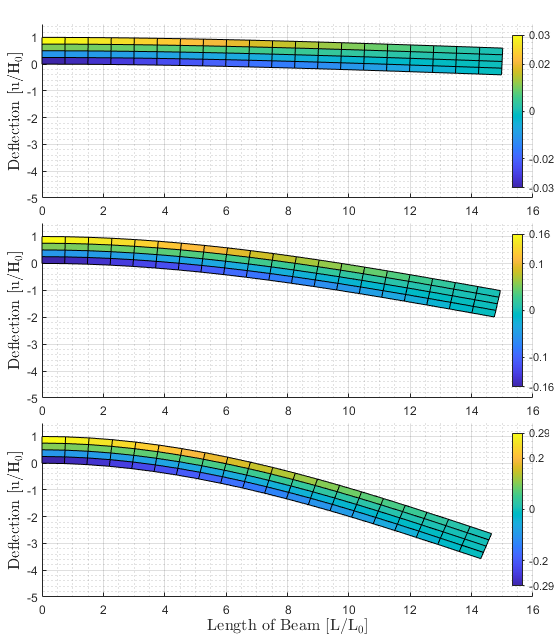
\includegraphics[height = 0.6\textheight, width = 0.5\paperwidth]{Images/beam_disp.png}
%        \hspace*{-2.9cm}
%        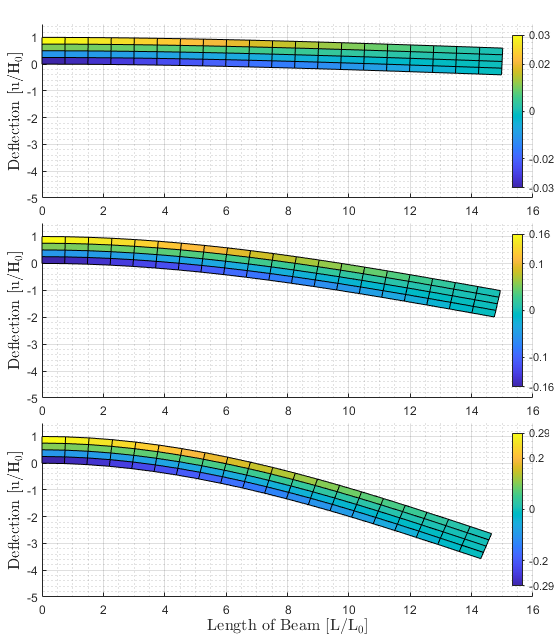
\includegraphics[scale = 0.7]{Images/beam_disp.png}
%        %\hspace{3.3cm}
%        \caption{Displacement driven boundary conditions}
%        \label{fig:beam_fe_disp}
%    \end{subfigure}
%    \hfill
%%    \begin{subfigure}[h]{0.48\textwidth} 
%        %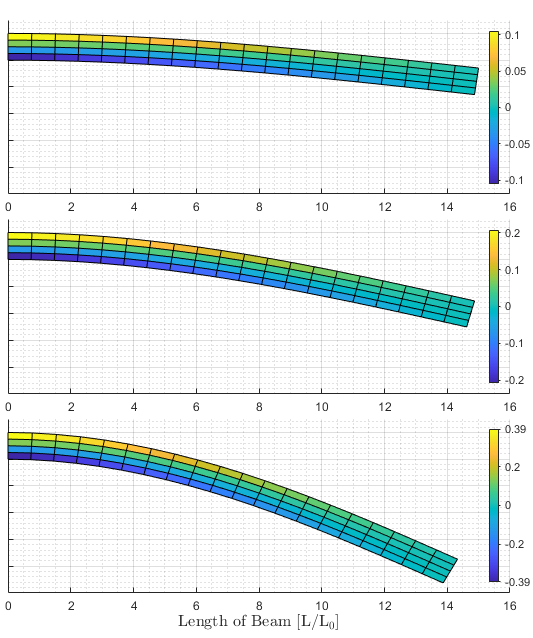
\includegraphics[height = 0.6\textheight, width = 0.5\paperwidth]{Images/beam_force.png}
%        %\hspace{0.25cm}
%        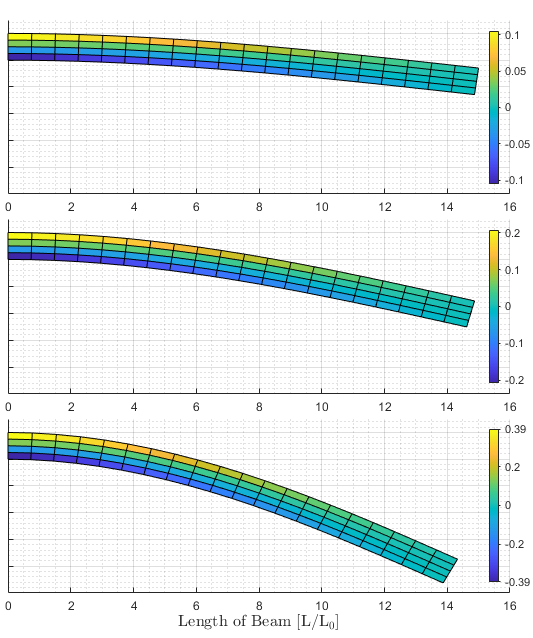
\includegraphics[scale = 0.7]{Images/beam_force.png}
%        %\captionsetup[subfigure]{oneside,margin={2cm,0cm}}
%        \caption{Force driven boundary conditions}
%        \label{fig:beam_fe_force}
%    \end{subfigure}
%    %\hspace*{\fill}
    
%    \caption{Numerical analysis of cantilever beam under various boundary conditions}
%    \label{fig:beam_fem}
%\end{figure}

\begin{figure}[h]
    \centering
    \begin{subfigure}{0.48\textwidth}
        \hspace*{-3cm}    
        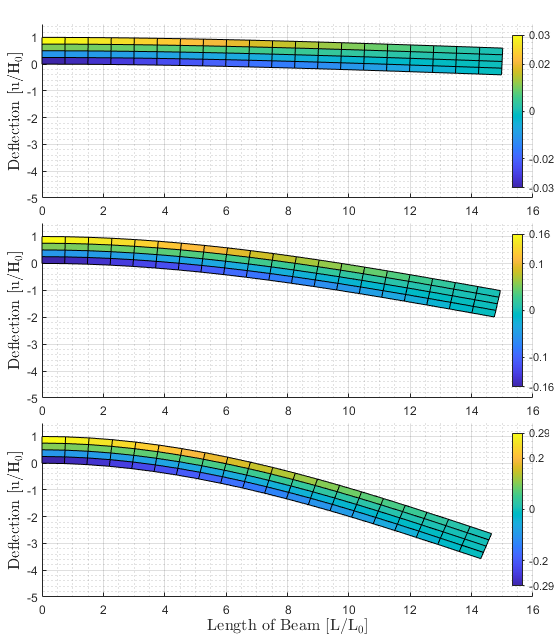
\includegraphics[scale = 0.70]{Images/beam_disp.png}
        \caption{Displacement driven boundary conditions}
        \label{fig:beam_fe_disp}
    \end{subfigure}
    \hfill
    \begin{subfigure}{0.48\textwidth}
        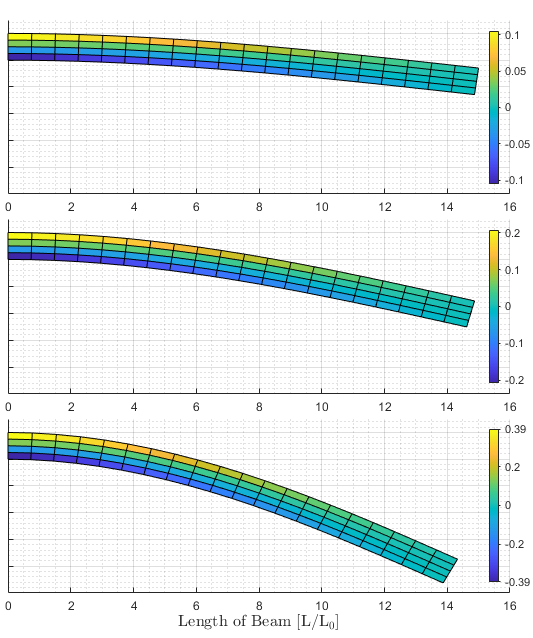
\includegraphics[scale=0.70]{Images/beam_force.png}
        \caption{Force driven boundary conditions}
        \label{fig:beam_fe_force}
    \end{subfigure}
    \caption[Numerical Analysis of Cantilever Beam]{Numerical analysis of cantilever beam under various boundary conditions}
    \label{fig:beam_fem}
\end{figure}